\documentclass{article}
\usepackage{graphicx} % Required for inserting images
\usepackage[left=1.5cm, right=1.5cm, top=1.5cm]{geometry}
\usepackage{enumitem}
\usepackage{amsmath}
\usepackage{amsfonts}
\usepackage[utf8]{inputenc}
\title{Distributed Systems: Assignment 1}
\author{Deven Mistry}
\date{January 31st, 2025}
\setlength\parindent{0pt}
\begin{document}

\maketitle

In this assignment, a simple `http.server' server was made in python to enable the client to send JSON messages to the server.

\section*{Server}

\begin{enumerate}
    \item The server then processes the JSON message and sends a response back to the client. The server was tested using the `python server.py' command in the terminal.
    \item The server has a MessageHandler class that processes the JSON message and sends a response back to the client.
\end{enumerate}

\section*{Client}

\begin{enumerate}
    \item The client sends a JSON message to the server. The client was tested using the `python client.py' command in the terminal.
    \item The client sends a JSON message to the server using the requests library using a POST method.
\end{enumerate}

\section*{Screenshot of the server and client}

\begin{figure}[h]
    \centering
    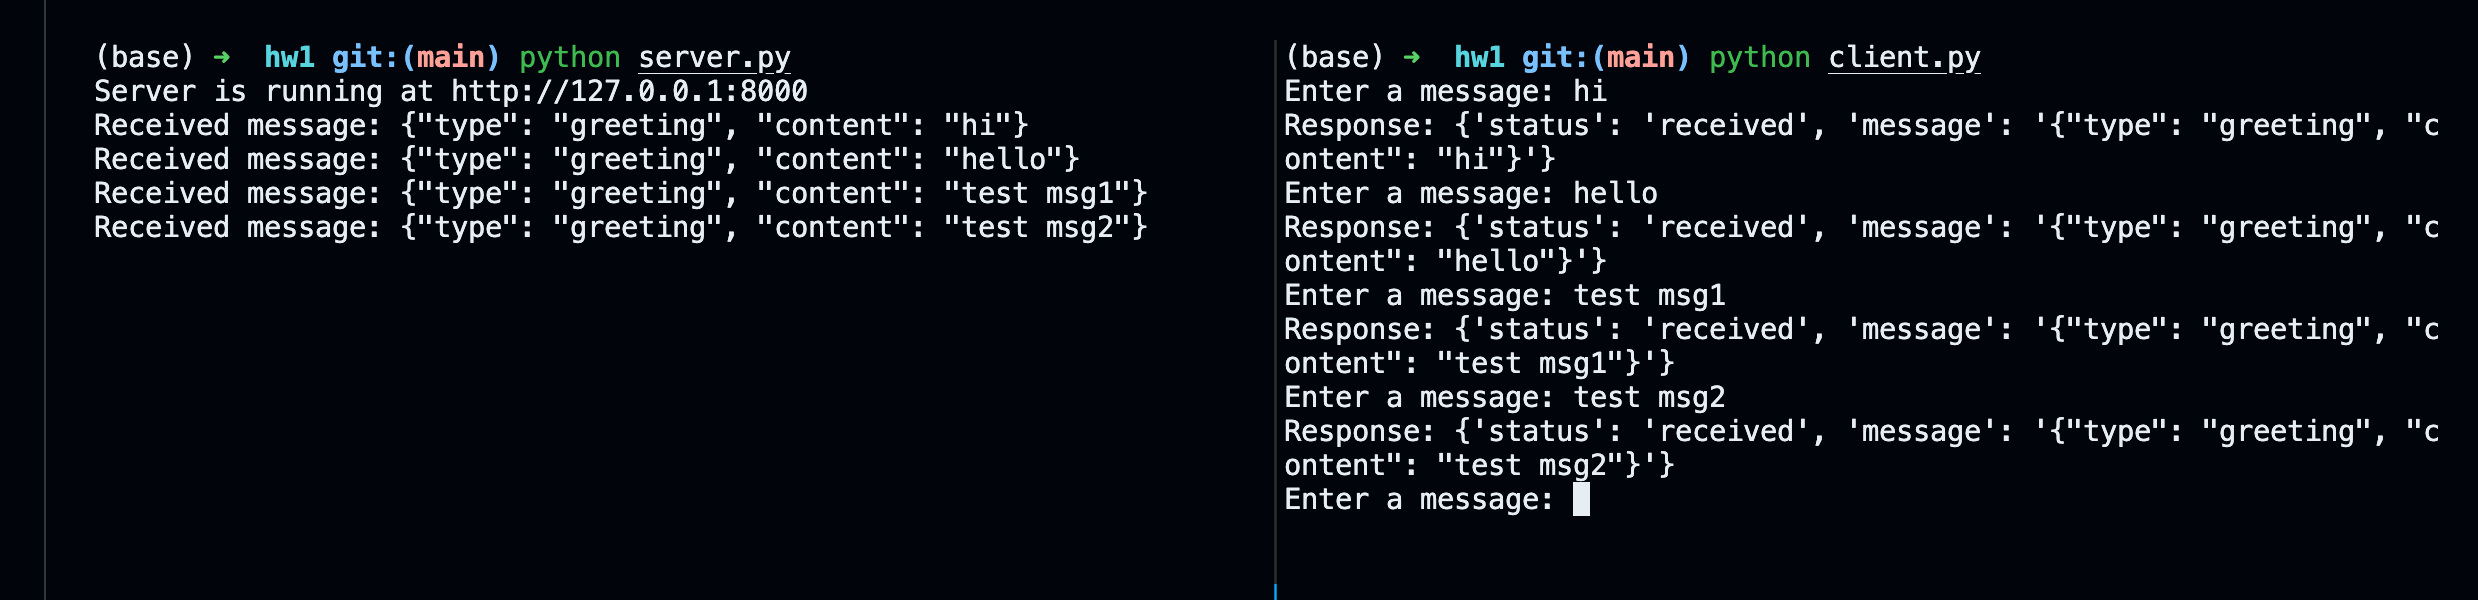
\includegraphics[width=0.8\textwidth]{image.png}
    \caption{Client server interaction}
\end{figure}

\end{document}